%\documentclass[twocolumn,traditabstract,referee]{aa}  
\documentclass[twocolumn,traditabstract]{aa}  

\usepackage{fixltx2e}
\usepackage[english]{babel}
\usepackage{graphicx,amsmath}
\usepackage{epstopdf}
\usepackage{epsf,color}
\usepackage[mathscr]{eucal}
\usepackage{amsmath}
\usepackage{amssymb,amsfonts}
\usepackage{natbib}
\usepackage{graphicx}
\usepackage{txfonts}
\usepackage{dsfont}
\definecolor{Mygreen}{rgb}{0.75, 0.0, 0.0}
\definecolor{Mypink}{rgb}{1.0, 0.0, 0.5}
\definecolor{Myred}{rgb}{0.7, 0.0, 0.0}
\usepackage[breaklinks, citecolor=blue, linkcolor=Myred, urlcolor=Myred, colorlinks=true, debug, baseurl=' ']{hyperref}
\usepackage{float} 
\usepackage{color}

\bibpunct{(}{)}{;}{a}{}{,}
\bibliographystyle{aa}

\begin{document}
%###############################################################################################
%##########################           START THE PAPER           ##########################################
%###############################################################################################
\title{Mapping the hot gas temperature in galaxy clusters using X-ray and Sunyaev-Zel'dovich imaging}
\author{R.~Adam \inst{\ref{OCA},\ref{LPSC},\ref{CEFCA}}\thanks{Corresponding author: R\'emi Adam, \url{remi.adam@oca.eu}}
\and O.~Hahn\inst{\ref{OCA}}						%NCT
\and  F.~Ruppin \inst{\ref{LPSC}}
\and  P.~Ade \inst{\ref{Cardiff}}
\and  P.~Andr\'e \inst{\ref{CEA}}
\and M.~Arnaud\inst{\ref{CEA}}					%NCT
\and I.~Bartalucci\inst{\ref{CEA}}					%NCT
\and  A.~Beelen \inst{\ref{IAS}}
\and  A.~Beno\^it \inst{\ref{Neel}}
\and  A.~Bideaud \inst{\ref{Neel}}
\and  N.~Billot \inst{\ref{IRAME}}
\and  O.~Bourrion \inst{\ref{LPSC}}
\and  M.~Calvo \inst{\ref{Neel}}
\and  A.~Catalano \inst{\ref{LPSC}}
\and  G.~Coiffard \inst{\ref{IRAMF}}
\and  B.~Comis \inst{\ref{LPSC}}
\and  A.~D'Addabbo \inst{\ref{Neel},\ref{Roma}}
\and  F.-X.~D\'esert \inst{\ref{IPAG}}
\and  S.~Doyle \inst{\ref{Cardiff}}
\and C.~Ferrari\inst{\ref{OCA}}						%NCT
\and  J.~Goupy \inst{\ref{Neel}}
\and  C.~Kramer \inst{\ref{IRAME}}
\and  G.~Lagache \inst{\ref{LAM}}
\and  S.~Leclercq \inst{\ref{IRAMF}}
\and  J.-F.~Lestrade \inst{\ref{LERMA}}
\and  J.F.~Mac\'ias-P\'erez \inst{\ref{LPSC}}
\and G.~Martinez Aviles\inst{\ref{OCA}}				%NCT
\and D.~Martizzi\inst{\ref{Berkeley}}					%NCT
\and S.~Maurogordato\inst{\ref{OCA}}				%NCT
\and  P.~Mauskopf \inst{\ref{Cardiff},\ref{Arizona}}
\and  F.~Mayet \inst{\ref{LPSC}}
\and  A.~Monfardini \inst{\ref{Neel}}
\and  F.~Pajot \inst{\ref{IAS}}
\and  E.~Pascale \inst{\ref{Cardiff}}
\and  L.~Perotto \inst{\ref{LPSC}}
\and  G.~Pisano \inst{\ref{Cardiff}}
\and E.~Pointecouteau\inst{\ref{IRAP}, \ref{UniToulouse}}%NCT
\and  N.~Ponthieu \inst{\ref{IPAG}}
\and G.W.~Pratt\inst{\ref{CEA}}					%NCT
\and  V.~Rev\'eret \inst{\ref{CEA}}
\and M.~Ricci\inst{\ref{OCA}}						%NCT
\and  A.~Ritacco \inst{\ref{IRAME}}
\and  L.~Rodriguez \inst{\ref{CEA}}
\and  C.~Romero \inst{\ref{IRAMF}}
\and  H.~Roussel \inst{\ref{IAP}}
\and  K.~Schuster \inst{\ref{IRAMF}}
\and  A.~Sievers \inst{\ref{IRAME}}
\and  S.~Triqueneaux \inst{\ref{Neel}}
\and  C.~Tucker \inst{\ref{Cardiff}}
\and H.-Y.~Wu\inst{\ref{CalTech}}					%NCT
\and  R.~Zylka \inst{\ref{IRAMF}}}

\institute{
  Laboratoire Lagrange, Universit\'e C\^ote d'Azur, Observatoire de la C\^ote d'Azur, CNRS, Blvd de l'Observatoire, CS 34229, 06304 Nice cedex 4, France
  \label{OCA}
  \and
  Laboratoire de Physique Subatomique et de Cosmologie, Universit\'e Grenoble Alpes, CNRS/IN2P3, 53, avenue des Martyrs, Grenoble, France
  \label{LPSC}
    \and
  Centro de Estudios de F\'isica del Cosmos de Arag\'on (CEFCA), Plaza San Juan, 1, planta 2, E-44001, Teruel, Spain
  \label{CEFCA}
  \and
Institut de RadioAstronomie Millim\'etrique (IRAM), Grenoble, France
  \label{IRAMF}
\and
Laboratoire AIM, CEA/IRFU, CNRS/INSU, Universit\'e Paris Diderot, CEA-Saclay, 91191 Gif-Sur-Yvette, France 
  \label{CEA}
\and
Astronomy Instrumentation Group, University of Cardiff, UK
  \label{Cardiff}
\and
Institut d'Astrophysique Spatiale (IAS), CNRS and Universit\'e Paris Sud, Orsay, France
  \label{IAS}
\and
Institut N\'eel, CNRS and Universit\'e Grenoble Alpes, France
  \label{Neel}
\and
Institut de RadioAstronomie Millim\'etrique (IRAM), Granada, Spain
  \label{IRAME}
\and
Dipartimento di Fisica, Sapienza Universit\`a di Roma, Piazzale Aldo Moro 5, I-00185 Roma, Italy
  \label{Roma}
\and
Univ. Grenoble Alpes, CNRS, IPAG, F-38000 Grenoble, France 
  \label{IPAG}
    \and
Aix Marseille Universit\'e, CNRS, LAM (Laboratoire d'Astrophysique de Marseille) UMR 7326, 13388, Marseille, France
  \label{LAM}
\and
School of Earth and Space Exploration and Department of Physics, Arizona State University, Tempe, AZ 85287
  \label{Arizona}
\and
Universit\'e de Toulouse, UPS-OMP, Institut de Recherche en Astrophysique et Plan\'etologie (IRAP), Toulouse, France
  \label{IRAP}
\and
CNRS, IRAP, 9 Av. colonel Roche, BP 44346, F-31028 Toulouse cedex 4, France 
  \label{IRAP2}
\and
University College London, Department of Physics and Astronomy, Gower Street, London WC1E 6BT, UK
  \label{UCL}
\and 
Institut d'Astrophysique de Paris, Sorbonne Universit\'es, UPMC Univ. Paris 06, CNRS UMR 7095, 75014 Paris, France 
  \label{IAP}
\and 
LERMA, CNRS, Observatoire de Paris, 61 avenue de l'Observatoire, Paris, France
  \label{LERMA}
  \and  
Department of Astronomy, University of California, Berkeley, CA 94720-3411, USA
  \label{Berkeley}
    \and
Universit\'e de Toulouse, UPS-OMP, Institut de Recherche en Astrophysique et Plan\'etologie (IRAP), Toulouse, France
  \label{IRAP}
\and
CNRS, IRAP, 9 Av. colonel Roche, BP 44346, F-31028 Toulouse cedex 4, France 
  \label{UniToulouse}
  \and
California Institute of Technology, MC 367-17, Pasadena, CA 91125, USA.
  \label{CalTech}  
}



\date{Received \today \ / Accepted --}
\abstract {We propose an alternative method to map the temperature distribution of the hot gas in galaxy clusters that uses resolved images of the thermal Sunyaev-Zel'dovich (tSZ) effect in combination with X-ray data. Application of the method to images from the New IRAM KIDs Array (NIKA) and XMM-\textit{Newton} allows us to measure the gas temperature and determine its spatial distribution in the merging cluster \mbox{MACS~J0717.5+3745}, at $z=0.55$.  Despite the complexity of the target cluster, we find a good morphological agreement between the temperature maps derived from X-ray spectroscopy only -- using XMM-\textit{Newton} ($T_{\rm XMM}$) and \textit{Chandra} ($T_{\rm CXO}$) -- and the new gas-mass-weighted tSZ+X-ray imaging method ($T_{\rm gmw}$). We correlate the temperatures from tSZ+X-ray imaging and those from X-ray spectroscopy alone, providing an independent temperature cross calibration. {\bf We find that $T_{\rm gmw}$ is higher than $T_{\rm XMM}$ and lower than $T_{\rm CXO}$, by $\sim 10\%$ in both cases.} Our results are limited by uncertainties in the geometry of the cluster gas and kinetic SZ contamination ($\sim 10\%$), and the absolute calibration of the tSZ map ($7\%$). Investigation using a larger sample of clusters would minimize these effects.}
\titlerunning{Mapping the temperature in galaxy clusters using X-ray and tSZ imaging}
\authorrunning{R. Adam, M. Arnaud, I. Bartalucci, et al.}
\keywords{Techniques: high angular resolution -- Galaxies: clusters: individual: \mbox{MACS~J0717.5+3745}; intracluster medium -- X-rays: galaxies: clusters}
\maketitle

%###############################################################################################
%##########################                             INTRODUCTION                              ##########################
%###############################################################################################
\section{Introduction}\label{sec:Introduction}
%Temperature is key for astro and cosmo
The temperature and density are the key observable characteristics of the hot ionized gas in the intracluster medium (ICM) of galaxy clusters. X-ray observations have historically played a fundamental role in their measurement: the density is trivial to obtain from X-ray imaging, while the temperature can be derived from an isothermal model fit to the spectrum. Accurate gas temperatures are needed for a number of reasons. They are essential to infer cluster masses under the assumption of hydrostatic equilibrium \citep{Sarazin1988}; in turn, these masses can be used to infer constraints on cosmological parameters \citep[e.g.,][]{Allen2011}. The temperature structure yields information on the detailed physics of shock-heated gas in merging events, the nature of cold fronts, and the role of turbulence and gas sloshing \citep[see, e.g.,][for a review]{mar07}. In turn, such analyses provide insights into the physics of galaxy clusters, which is necessary to interpret the scaling relations between clusters masses and their primary observables \citep{Khedekar2013}.

%Difficulties in measurments
However, the X-ray gas temperature measurement is potentially affected by two systematic effects. First, the X-ray emission is proportional to the square of the ICM electron density, such that spectroscopic temperatures are driven by the colder,  denser, regions along the line-of-sight, and are thus sensitive to gas clumping. What is measured is in fact a weighted mean temperature, where the weight is a non-linear combination of the temperature and density structure \citep[see, e.g.,][]{maz04,vik06b}. Numerical simulations support this view \citep[e.g.,][]{Nagai2007,ras14}, but estimates of the magnitude of any bias due to this effect vary widely depending on the numerical scheme (e.g., smoothed particle hydrodynamics, adaptive mesh refinement) and the details of the `sub-grid' physics (cooling, feedback, etc). Secondly, the spectroscopic temperatures depend directly on the energy calibration of X-ray observatories. For instance, X-ray temperatures obtained with \textit{Chandra} are generally higher than those measured by XMM-\textit{Newton}, by up to a factor of 15\% at 10~keV \citep[e.g.,][]{Mahdavi2013}.

%SZ can help
The thermal Sunyaev-Zel'dovich \citep[tSZ,][]{Sunyaev1972} effect is related to the mean gas-mass-weighted temperature along the line-of-sight and the electron density, via the ideal gas law. The tSZ effect can thus be used to obtain an alternative estimate of the gas temperature, provided a measure of the density is available. Combination of the tSZ and X-ray observations can then in principle be used to decouple temperature and density in each individual measurement. {\bf Several groups have already attempted to extract the gas temperature distribution in one dimension using such method, complementing X-ray spectroscopic measurements. See for instance \cite{Pointecouteau2002,Kitayama2004,Nord2009,Basu2010,Eckert2013,Ruppin2016}.}

%What we do and do not do here
Here we use deep, resolved ($< 20\arcsec$) tSZ observations, combined with X-ray imaging, to measure the spatial distribution of the gas temperature toward the merging cluster \mbox{MACS~J0717.5+3745} at $z=0.55$, {\bf in two dimensions}. We have chosen \mbox{MACS~J0717.5+3745} because it is one of the very few objects for which sufficiently deep and resolved tSZ data are currently available \citep{Adam2016b}. The complex morphology of the cluster is the primary limiting factor to our analysis; however it allows us to explore a wide range of gas temperatures, which will not necessarily be accessible with more simple objects. {\bf The aim of this paper is thus to explore a new method to reconstruct the spatial distribution of the hot gas temperature in galaxy clusters, base on X-ray and tSZ imaging, using a test case cluster. We compare it to the classical X-ray spectroscopic technique using XMM-\textit{Newton} and \textit{Chandra} data, but as our results are limited by systematic effects, we do not aim at favoring one X-ray measurement over the other.}

%Planck cosmology
We assume a flat $\Lambda$CDM cosmology according to the latest {\it Planck} results \citep{Planck2015XIII} with $H_0 = 67.8$ km s$^{-1}$ Mpc$^{-1}$, $\Omega_M = 0.308$, and $\Omega_{\Lambda} = 0.692$. At the cluster's redshift, 1 arcsec corresponds to 6.6 kpc.

%###############################################################################################
%##########################                                        Data                                      ##########################
%###############################################################################################
\section{Data}\label{sec:data}
%========== SZ data
The New IRAM KIDs Array \citep[NIKA, see][]{Monfardini2011,Calvo2013,Adam2014,Catalano2014} has observed \mbox{MACS~J0717.5+3745} at 150 and 260 GHz for a total of 47.2 ks. The main steps of the data reduction are described in \cite{Adam2015,Adam2016a,Adam2016b,Ruppin2016}. In this paper, we use the NIKA 150 GHz tSZ map at 22 arcsec effective angular resolution FWHM, deconvolved from the transfer function except for the beam smoothing. The overall calibration uncertainty is estimated to be 7\%, including the brightness temperature model of our primary calibrator, the NIKA bandpass uncertainties, the opacity correction, and the stability of the instrument \citep{Catalano2014}. The absolute zero level for the brightness on the map remains unconstrained by NIKA. \mbox{MACS~J0717.5+3745} is contaminated by a significant amount of kinetic SZ \citep[kSZ,][]{Sunyaev1980} signal and we used the best-fit model F2 from \cite{Adam2016b} to remove its contribution. This model has large uncertainties but it still allows us to test the impact of the kSZ effect on our results.

%========== XMM/Chandra
\mbox{MACS~J0717.5+3745} was observed several times by the XMM-\textit{Newton} and \textit{Chandra} X-ray observatories (obs-IDs 0672420101, 0672420201, 067242030, and {\bf 1655, 4200, 16235, 16305}, respectively). The data processing follows the description given in \cite{Adam2016b}. The clean exposure time is 153 ks for \textit{Chandra} and 160 and 116 ks for XMM-\textit{Newton} MOS1,2 and PN cameras, respectively.

%###############################################################################################
%##########################                                     Method                                     ##########################
%###############################################################################################
\section{Temperature reconstruction}\label{sec:method}
{\bf The method employed to recover the temperature of the gas from NIKA tSZ and XMM-\textit{Newton} X-ray imaging, $\bar{T}_{\rm gmw}$, is described below. We also discuss the X-ray spectroscopic temperature mapping in Section \ref{sec:Xray_spectroscopic_temperature_map}, which we use for comparison in Section \ref{sec:compT}.}

%========== Primary observables
\subsection{Primary observables}
The tSZ signal, measured at frequency $\nu$, can be expressed as
\begin{equation}
	\frac{\Delta I_{\nu}}{I_0} =  f(\nu, T_e) \frac{\sigma_{\rm T}}{m_e c^2} \int P_e dl \equiv k_{\rm B} \bar{T}_{\rm gmw} f(\nu, T_e) \frac{\sigma_{\rm T}}{m_e c^2} \int n_e dl,
\label{eq:dIsz}
\end{equation}
where $f(\nu, T_e)$ is the tSZ spectrum, which depends slightly on temperature $T_e$ in the case of very hot gas. The signal is proportional to the line-of-sight integrated electron pressure, $P_{e}$. It is related to the mean gas-mass-weighted temperature along the line-of-sight, 
\begin{equation}
        \bar{T}_{\rm gmw} \equiv \frac{\int T_e n_e dl}{\int n_e dl},
        \label{eq:Tgmw_def}
\end{equation}
and the electron density, $n_e$, via the ideal gas law. The X-ray surface brightness is driven by the electron density:
\begin{equation}
        S_{\rm X}= \frac{1}{4 \pi \left(1+z\right)^4} \int n_e^2 \Lambda(T_e, Z) \ dl,
        \label{eq:sx}
\end{equation}
where  $z$ is the cluster redshift, and $\Lambda(T_e, Z)$ is the emissivity in the relevant energy band, taking into account the interstellar absorption and the instrument spectral response. $\Lambda(T_e, Z)$ depends only weakly on the temperature and metallicity of the gas $Z$, so that instrumental systematics have a negligible impact on the results presented in this paper.

%========== Density from X-ray
\subsection{X-ray electron density mapping}
We use the XMM-\textit{Newton} X-ray surface brightness (equation \ref{eq:sx}) to produce a map of the square of the electron density integrated along the line-of-sight. To combine it with tSZ observations, we have to convert $\int n_e^2 dl$ to $\int n_e dl$ via an effective electron depth, expressed as
\begin{equation}
	\ell_{\rm eff} = \frac{\left(\int n_e dl\right)^2}{\int n_e^2 dl}.
\label{eq:l_eff}
\end{equation}
From equation~\ref{eq:sx}, the effective electron density along the line-of-sight is then given by
\begin{equation}
	\bar{n}_e = \frac{1}{\ell_{\rm eff}} \int n_e dl = \frac{1}{\ell_{\rm eff}}\sqrt{\ell_{\rm eff} \frac{4 \pi \left(1+z\right)^4 S_{\rm X}}{\Lambda\left(T_e, Z\right)}}.
\label{eq:pseudo_ne}
\end{equation}
We use several approaches to estimate $\ell_{\rm eff}$ and its uncertainty:
\begin{enumerate}
\item {\bf Model M1} Following \cite{Sayers2013}, we assume that $\ell_{\rm eff}$ is constant at $\ell_{\rm eff}=1400$ kpc, as estimated by \citet{Mroczkowski2012}, across the cluster extension. 
\item {\bf Model M2} We derive an electron density profile from deconvolution and deprojection of the XMM-\textit{Newton} radial $S_{\rm X}$ profile centered on the X--ray peak \citep{Croston2006}, thus obtaining an azimuthally symmetric $\ell_{\rm eff}$ map. 
\item {\bf Model M3} We use the best fitting NIKA tSZ+XMM-\textit{Newton} density model of \cite{Adam2016b}, which accounts for the four main subclusters in \mbox{MACS~J0717.5+3745}, to compute a map of $\ell_{\rm eff}$. The model does not constrain the line-of-sight distance between the subclusters because the tSZ signal depends linearly on the density. Therefore, we consider two extreme cases: {\bf M3a)} where the subclusters are sufficiently far away from each other such that $\int n_e^2 dl \simeq \sum_j \int n_{e,j}^2 dl$, where $j$ refers to each subcluster; {\bf M3b)} where all the subclusters are located {\bf in the same plane, perpendicular to the line-of-sight. They have thus the same line-of-sight coordinate, i.e. the same redshift, such that the physical distance between the subclusters are minimal.}
\end{enumerate}
The internal structure of \mbox{MACS~J0717.5+3745} is increasingly refined from model M1 to M3, but we find good consistency between all three models. Model M2 presents a minimum of 1200 kpc toward the X-ray center and increases quasi-linearly toward higher radii, reaching about 2000 kpc at 1 arcmin, in line with expectations from model M1. Model M3a is minimal in the central region, in the direction of the subclusters ($\sim 1200$ kpc), and also increases with radius. Model M3b provides a lower limit for $\ell_{\rm eff}$, increasing from $\sim 800$ kpc near the center to $\sim 1200$ kpc at 1 arcmin. 

{\bf The electron depth is related to the geometry and to the clumping of the gas. While our models allow us to test the impact of the gas geometry on large scales, it does not account specifically for clumping on small scales. Despite the weak dependance of the gas-mass-weighted temperature on the electron depth, ($\propto \sqrt{\ell_{\rm eff}}$), clumping might affect our results as discussed in Section \ref{sec:conclusions}.

The left panel of Figure \ref{fig:Input_maps} represents the $\bar{n}_e$ map in the case of model M1, thus $\propto \sqrt{\int n_e^2 dl}$. The cluster clearly exhibits a disturbed morphology. The gas roughly follows the four main substructures identified in the galaxy distribution \citep{Ma2009}.}

%========== Pressure from tSZ
\subsection{Thermal Sunyaev-Zel'dovich pressure mapping}
We can express the effective pressure along the line-of-sight directly from equation \ref{eq:dIsz}, as
\begin{equation}
	\bar{P_e} = \frac{1}{\ell_{\rm eff}} \int P_e dl = \frac{m_e c^2}{\sigma_{\rm T}} \frac{y_{\rm tSZ}}{\ell_{\rm eff}}.
\label{eq:pseudo_p}
\end{equation}
This quantity is straightforwardly obtained from the NIKA map accounting for relativistic corrections as detailed in \cite{Adam2016b}. As the temperature can be very high, the relativistic corrections are non negligible \citep{Pointecouteau1998,Itoh2003}, but the exact choice of the temperature map used to apply relativistic corrections has a negligible impact on our results {\bf (i.e., the spectroscopic temperature maps from XMM-\textit{Newton}, from \textit{Chandra},  or $\bar{T}_{\rm gmw}$)}. The right panel of Figure \ref{fig:Input_maps} presents the $\bar{P}_e$ map in the case of model M1, {\bf thus $\propto \int P_e dl$, corrected} for kSZ and zero level (see Section \ref{sec:compT}). {\bf The pressure distribution also indicates that the cluster is disturbed. The morphology is similar to that of the density on large scales, but we observe strong differences at the substructure level, which indicate spatial variations of the temperature. We note in particular that the pressure peak is offset $\sim 30$ arcsec southeast with respect to the density peak.}

\begin{figure*}[h]
\centering
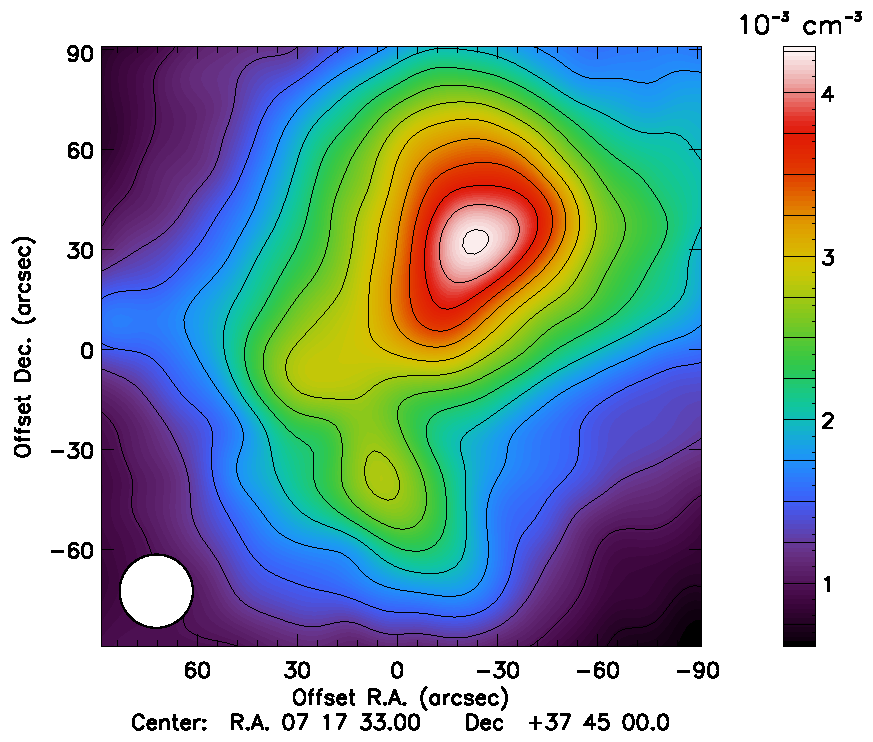
\includegraphics[height=7.6cm]{Figure/Thermo_N1.pdf}
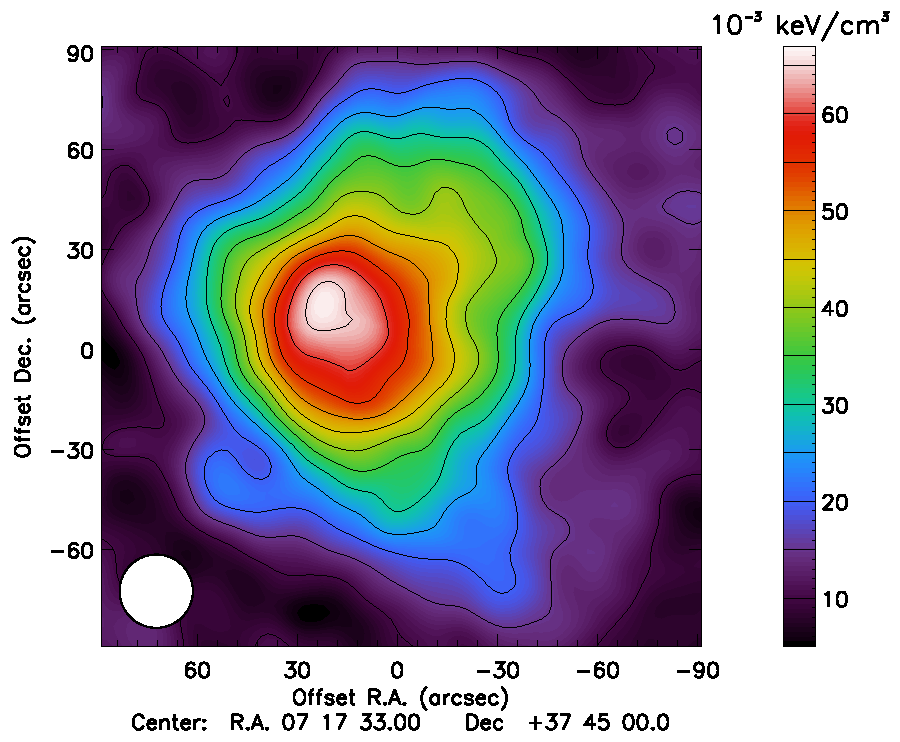
\includegraphics[height=7.6cm]{Figure/Thermo_Pclean1.pdf}
\caption{\footnotesize{{\bf Left}: effective line-of-sight integrated electron density, $\bar{n}_e$, derived from XMM-\textit{Newton}. {\bf Right}: effective line-of-sight integrated pressure, $\bar{P}_e$, derived from NIKA. These maps correspond to model M1, and were smoothed with a Gaussian kernel to an effective resolution of 22 arcsec FWHM. The pressure map is cleaned from our best-fit kSZ model and corrected for the zero level.}}
\label{fig:Input_maps}
\end{figure*}

%========== Temperature
\subsection{Gas-mass-weighted temperature mapping}
The tSZ+X-ray imaging temperature map, referred to as gas-mass-weighted, is obtained by combining the effective density and the effective pressure: 
\begin{equation}
	k_{\rm B} \bar{T}_{\rm gmw} \equiv \frac{\int k_{\rm B} T_e n_e dl}{\int n_e dl} = \frac{\bar{P_e}}{\bar{n_e}} = \frac{m_e c^2}{\sigma_{\rm T}} \sqrt{\frac{\Lambda\left(T_e, Z\right)}{4 \pi \left(1+z\right)^4 \ell_{\rm eff} S_{\rm X}}} y_{\rm tSZ}.
\label{eq:pseudo_tsz}
\end{equation}
We propagate the noise arising from the tSZ map and the X-ray surface brightness using Monte Carlo realizations; the overall noise on $\bar{T}_{\rm gmw}$ is dominated by that of the tSZ map.

\begin{figure*}[h]
\centering
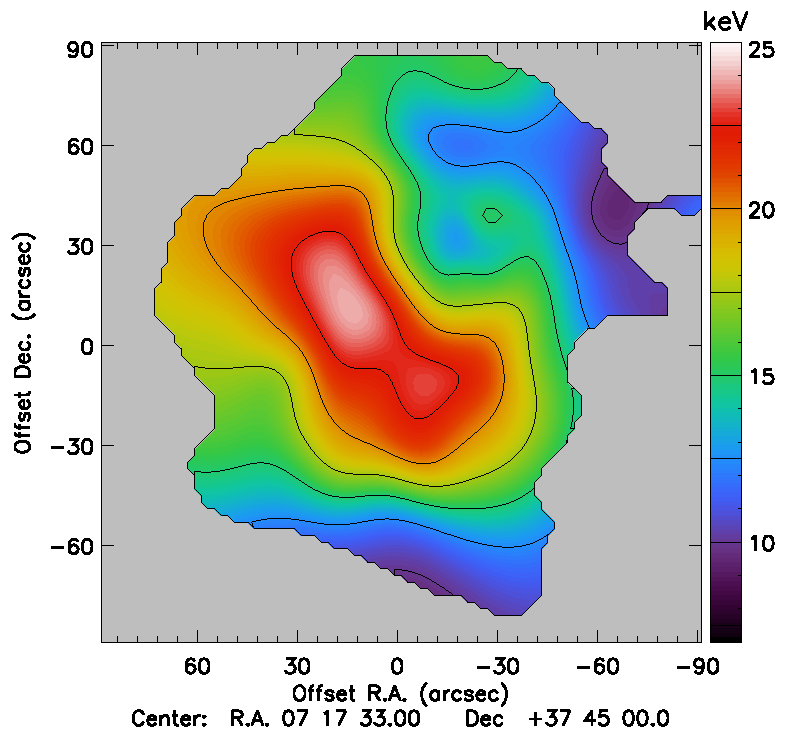
\includegraphics[trim=0cm 0cm 1.4cm 0cm, clip=true, totalheight=6.7cm]{Figure/Thermo_TCXO.pdf}
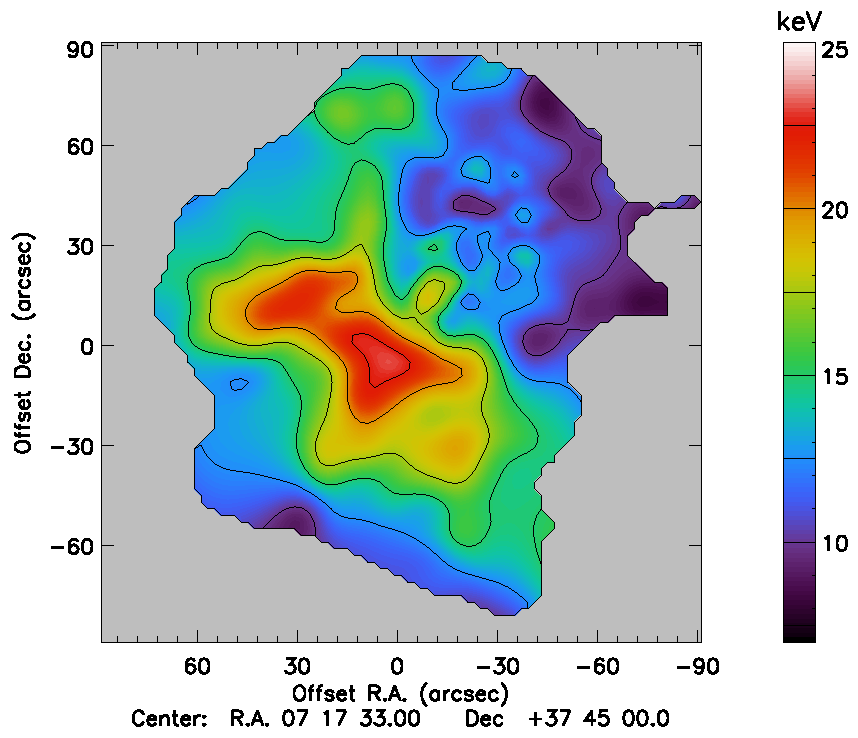
\includegraphics[trim=1.6cm 0cm 1.4cm 0cm, clip=true, totalheight=6.7cm]{Figure/Thermo_TXMM.pdf}
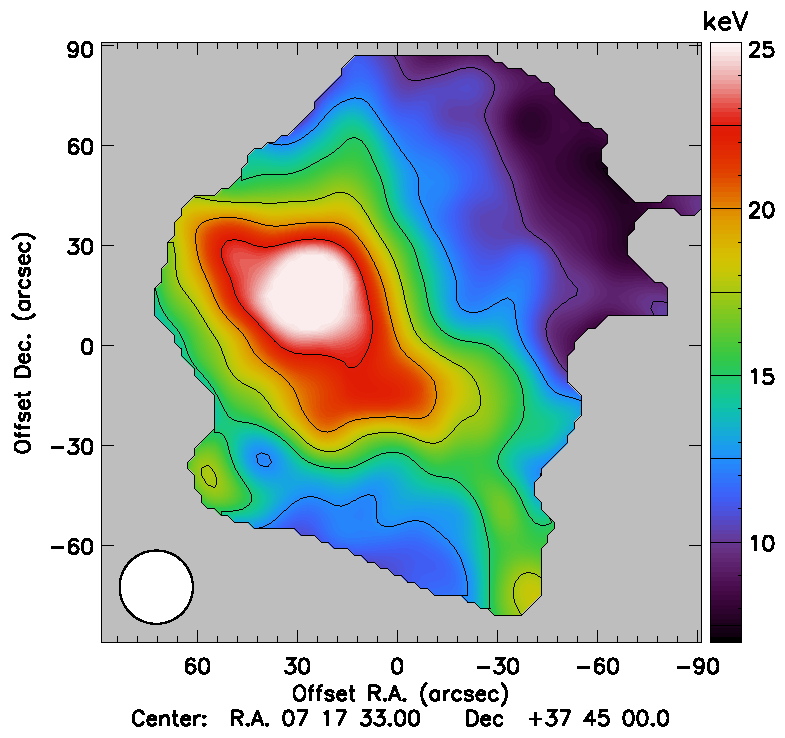
\includegraphics[trim=1.6cm 0cm 0cm 0cm, clip=true, totalheight=6.7cm]{Figure/Thermo_TSZclean1.pdf}
\caption{\footnotesize{{\bf Left}: \textit{Chandra} derived spectroscopic temperature map, $\bar{T}_{\rm CXO}$. {\bf Middle}: XMM-\textit{Newton} derived spectroscopic temperature map, $\bar{T}_{\rm XMM}$. {\bf Right}: NIKA+XMM-\textit{Newton} imaging derived temperature map for model M1, $\bar{T}_{\rm gmw}$. This map is corrected for the zero level.}}
\label{fig:T_maps}
\end{figure*}

%========== Spectro
\subsection{X-ray spectroscopic temperature map}\label{sec:Xray_spectroscopic_temperature_map}
{\bf The X-ray spectroscopic temperature maps from \textit{Chandra} ($\bar{T}_{\rm CXO}$) and XMM-\textit{Newton} ($\bar{T}_{\rm XMM}$) were produced using the wavelet filtering algorithm described in \cite{Bourdin2008}, as detailed in \cite{Adam2016b}. As the significance of wavelet coefficients partly depends on the photon count statistics, the effective resolution varies across the map, XMM-\textit{Newton} allowing a finer sampling than \textit{Chandra} due to the higher effective area. We estimate the uncertainties per map pixel using a Monte Carlo approach.} \textcolor{red}{Do you want to discuss in more details the Monte Carlo approach?}

%###############################################################################################
%##########################                                       Results                                   ##########################
%###############################################################################################
\section{Results}\label{sec:results}
%========== Morphology
\subsection{Morphology}
Figure \ref{fig:T_maps} shows the three temperature maps $\bar{T}_{\rm CXO}$, $\bar{T}_{\rm XMM}$, and $\bar{T}_{\rm gmw}$ for model M1. $\bar{T}_{\rm gmw}$ is kSZ-corrected, and corrected for the zero level. They all identify a hot gas `bar' to the southeast. The position of the temperature peak is the same for $\bar{T}_{\rm CXO}$ and $\bar{T}_{\rm gmw}$, while it is slightly shifted southwest for $\bar{T}_{\rm XMM}$; however it also coincides with a region where kSZ contamination is large, leading to possible overestimation in $\bar{T}_{\rm gmw}$. All three maps indicate cooler temperatures in the  the northwest sector. Varying the kSZ correction and the $\ell_{\rm eff}$ models slightly changes the morphology of $\bar{T}_{\rm gmw}$ locally, but the agreement with X-ray spectroscopy is good in all cases.

%========== Cross calibration
\subsection{Temperature comparison}\label{sec:compT}
\begin{figure*}[h]
\centering
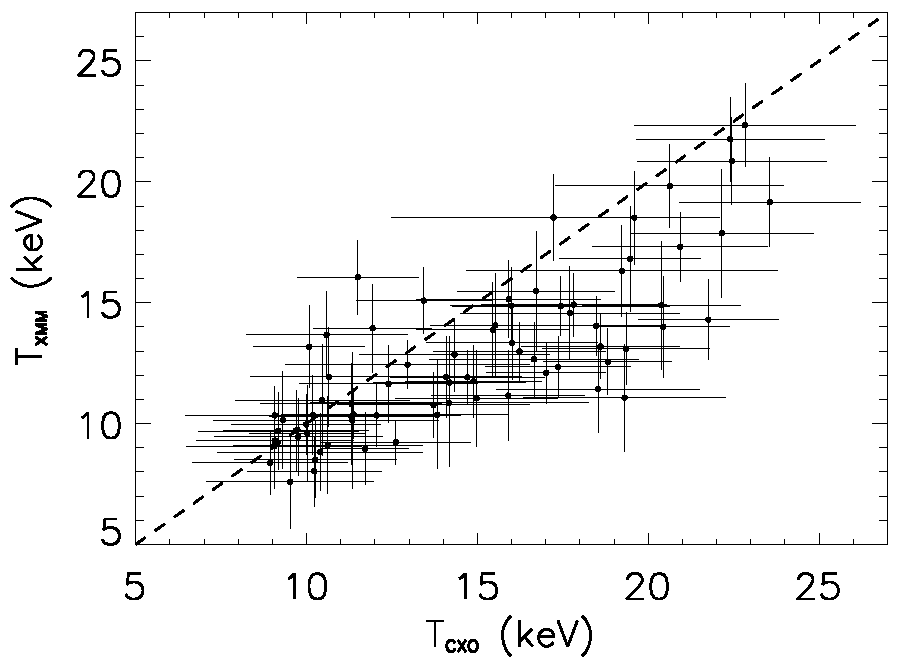
\includegraphics[width=0.33\textwidth]{Figure/Thermo_correlation_TXMM-TCXO.pdf}
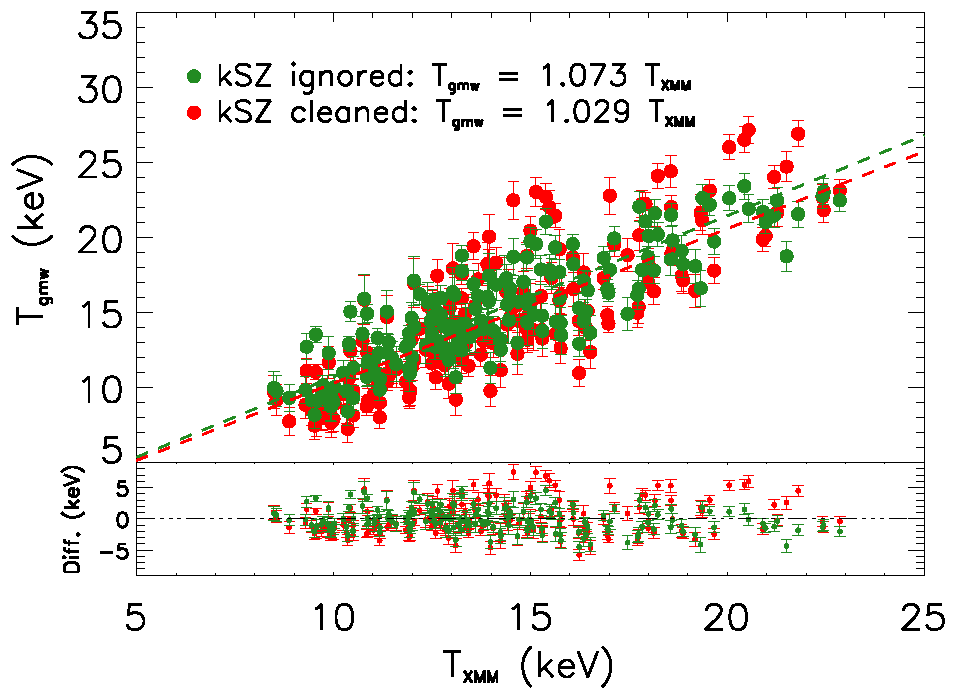
\includegraphics[width=0.33\textwidth]{Figure/Thermo_correlation_TXMM-TSZ_leff1.pdf}
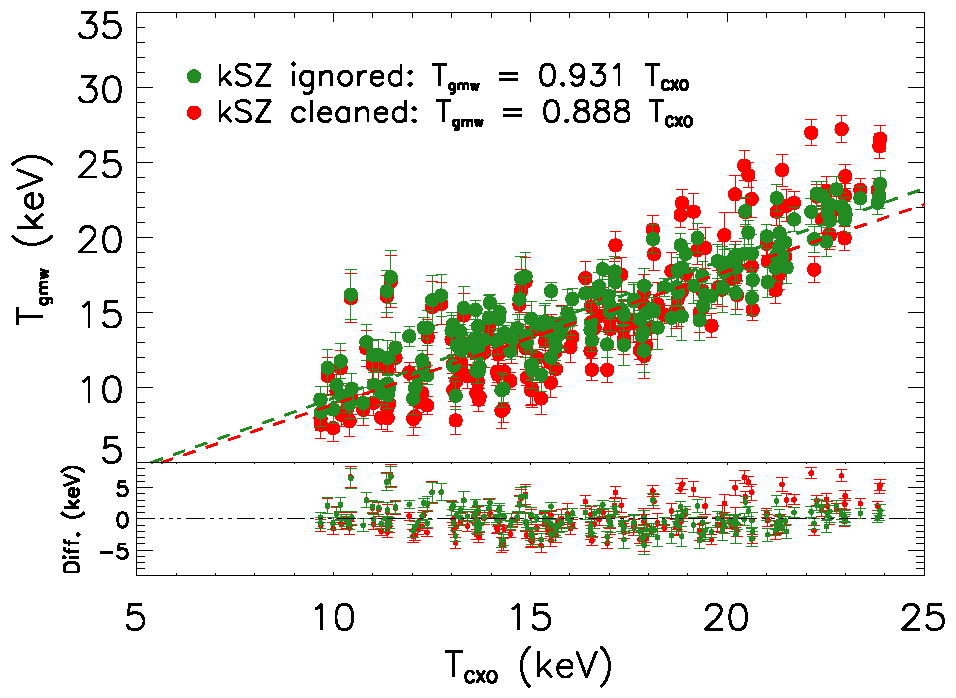
\includegraphics[width=0.33\textwidth]{Figure/Thermo_correlation_TCXO-TSZ_leff1.pdf}
\caption{\footnotesize{Correlation between the temperature maps of Figure \ref{fig:T_maps} and residual, $\chi^{(i)} = \frac{k_{\rm B} \bar{T}^{(i)}_{1} - \alpha \ k_{\rm B} \bar{T}^{(i)}_{2} - {\beta}/{\bar{n_e}^{(i)}}}{\sqrt{\left(\delta^{(i)}_{T_{1}}\right)^2 + \left(\alpha \ \delta^{(i)}_{T_{2}}\right)^2}}$. {\bf Left:} XMM-\textit{Newton} versus \textit{Chandra} spectroscopic temperatures. {\bf Middle:} tSZ+X-ray imaging (model M1) versus XMM-\textit{Newton} spectroscopy. {\bf Right:} tSZ+X-ray imaging (model M1) versus \textit{Chandra} spectroscopy. The red and green dots correspond to the case with and without the kSZ correction, respectively.}}
\label{fig:T_SZ_T_X_correlation}
\end{figure*}

Figure \ref{fig:T_SZ_T_X_correlation} shows the correlation between the maps shown in Figure \ref{fig:T_maps}. The temperature values are extracted in each {\bf 20} arcsec pixel, where the resolution of the $\bar{T}_{\rm gmw}$ map is 22 arcsec. We mask pixels where the tSZ signal-to-noise ratio is lower than 2 to avoid possible bouncing effects on the edge of the map due to the NIKA data processing.

Since the zero level of the tSZ map is unconstrained, we express the effective pressure map as $\bar{P}_e = \bar{P}_{\rm true} + \bar{P}_0$, where $\bar{P}_0$ is an unknown offset. Following equation \ref{eq:pseudo_tsz}, the gas-mass-weighted temperature can then be expressed with respect to the spectroscopic temperature, as
\begin{equation}
k_{\rm B} \bar{T}_{\rm gmw} = \alpha_{\rm gmw-X} \times k_{\rm B} \bar{T}_{\rm XMM/CXO} + {\beta}/{\bar{n_e}},
\label{eq:TSZ_TX_regression}
\end{equation}
where $\alpha_{\rm gmw-X}$ is a cross-calibration term and $\beta$ gives a measurement of $\bar{P}_0$. For X-ray spectroscopic temperatures, we simply write $\bar{T}_{\rm XMM} = \alpha_{\rm XMM-CXO} \times \bar{T}_{\rm CXO}$. 

{\bf We perform a linear regression between the pairs of temperature maps ($\bar{T}_{1,2} \equiv \bar{T}_{\rm XMM}, \bar{T}_{\rm CXO}, \bar{T}_{\rm gmw}$) accounting for error bars on both axis. To do so, we follow \cite{Orear1982} and define the following likelihood, $\mathscr{L}$, as
\begin{equation}
2 \ {\rm ln} \ \mathscr{L} = \sum_{i=1}^{N_{\rm pix}} \frac{\left(k_{\rm B} \bar{T}^{(i)}_{1} - \alpha \ k_{\rm B} \bar{T}^{(i)}_{2} - {\beta}/{\bar{n_e}^{(i)}}\right)^2}{\left(\delta^{(i)}_{T_{1}}\right)^2 + \left(\alpha \ \delta^{(i)}_{T_{2}}\right)^2},
\label{eq:chi2_def}
\end{equation}
where $\delta_{T_{1,2}}$ represents the temperature maps uncertainties and $\beta$ is set to zero when the regression is performed between $\bar{T}_{\rm XMM}$ and $\bar{T}_{\rm CXO}$. The parameter space is sampled using Markov Chains, which we evolve according to the Metropolis-Hasting algorithm \citep{Chib1995}, as done in \cite{Adam2015}. We check that this method correctly reproduce the true posterior likelihood using Monte Carlo realizations. Following \citep{Pratt2009}, we compute the overall scatter as
\begin{equation}
\sigma_{\rm tot}^2 = \frac{\frac{1}{N_{\rm pix} - 2} \sum_i \frac{\left(k_{\rm B} \bar{T}^{(i)}_{1} - \alpha \ k_{\rm B} \bar{T}^{(i)}_{2} - {\beta}/{\bar{n_e}^{(i)}}\right)^2}{\left(\delta^{(i)}_{T_{1}}\right)^2 + \left(\alpha \ \delta^{(i)}_{T_{2}}\right)^2}}{\frac{1}{N_{\rm pix}} \sum_i \frac{1}{\left(\delta^{(i)}_{T_{1}}\right)^2 + \left(\alpha \ \delta^{(i)}_{T_{2}}\right)^2}},
\label{eq:scatter_def}
\end{equation}
from which we extract the intrinsic scatter, $\sigma_{\rm int} = \sqrt{\sigma_{\rm tot}^2 - \sigma_{\rm stat}^2}$, accounting for the statistical scatter $\sigma_{\rm stat}$.}

Table~\ref{tab:regression_coeff} gives the $\alpha $ {\bf and $\beta$} coefficients {\bf and the intrinsic scatter}, obtained for the different $\ell_{\rm eff}$ models tested, and their dependence on the kSZ correction. {\bf Figure \ref{fig:T_SZ_T_X_posterior} provides the posterior likelihood in the plane $\alpha_{\rm gmw-X}$--$\beta$ for all the regression performed between $\bar{T}_{\rm gmw}$ and $\bar{T}_{\rm XMM/CXO}$.}

The scatter of about 2 keV between $\bar{T}_{\rm CXO}$ and $\bar{T}_{\rm XMM}$ is dominated by statistical error. The scatters between $\bar{T}_{\rm gmw}$ and both X-ray temperatures are comparable, {\bf but slightly lower for $\bar{T}_{\rm XMM}$}. This is not compatible with the noise as propagated into the $T_{\rm gmw}$ map {\bf in most cases}, and may be due to a number of factors, including the difference in angular resolution of the maps, or an intrinsic scatter between gas-mass-weighted and spectroscopic temperatures.

The tSZ+X-ray imaging versus X-ray only cross-calibration is stable to within 10\%, depending on the choice of the $\ell_{\rm eff}$ model and the kSZ correction used. The cross-calibration coefficients also directly depend on the absolute calibration of the tSZ map, which is expected to be accurate within 7\%. Model M3b provides a lower limit on $\ell_{\rm eff}$, and therefore an upper limit on $\alpha_{\rm gmw-X}$.

\begin{table*}[]
\caption{\footnotesize{Regression and {\bf intrinsic} scatter coefficients between the temperature maps. {\bf The central value is the median of the posterior likelihood and the errors are obtained by integrating the posterior likelihood within 90\% C.L. The posterior likelihood distribution is highly non Gaussian in the case of the scatter and error bars should be interpreted with caution.} $^{\star}$Model M3b gives a lower limit for $\ell_{\rm eff}$, and thus should be taken only as an upper limit for $\alpha$.}}
\begin{center}
\resizebox{\textwidth}{!} {
\begin{tabular}{c|ccc|c}
\hline
\hline
 & \multicolumn{4}{c}{$\ell_{\rm eff}$ model} \\
Slope / offset (mJy/Beam) / scatter (keV) & M1 & M2 & M3a & M3b$^{\star}$ \\
\hline
 & \multicolumn{4}{c}{kSZ-uncorrected} \\
\hline
$\left( \alpha, \beta, \sigma_{\rm int} \right)_{\rm gmw-XMM}$ & $\left(1.11_{-0.07}^{+0.08} , 1.04_{-0.10}^{+0.10} , 1.43_{-0.62}^{+0.38}\right)$ & $\left(1.06_{-0.07}^{+0.07} , 1.28_{-0.12}^{+0.12} , 1.29_{-0.60}^{+0.35}\right)$ & $\left(1.15_{-0.08}^{+0.08} , 1.17_{-0.11}^{+0.12} , 1.59_{-0.55}^{+0.37}\right)$ & $\left(1.70_{-0.12}^{+0.13} , 1.36_{-0.14}^{+0.14} , 2.44_{-0.71}^{+0.50}\right)$ \\
$\left( \alpha, \beta, \sigma_{\rm int} \right)_{\rm gmw-CXO}$ & $\left(0.90_{-0.07}^{+0.07} , 0.93_{-0.10}^{+0.11} , 1.59_{-0.78}^{+0.47}\right)$ & $\left(0.85_{-0.06}^{+0.07} , 1.12_{-0.12}^{+0.13} , 1.51_{-0.67}^{+0.41}\right)$ & $\left(0.90_{-0.07}^{+0.08} , 1.01_{-0.11}^{+0.12} , 2.51_{-0.40}^{+0.36}\right)$ & $\left(1.39_{-0.11}^{+0.14} , 1.23_{-0.13}^{+0.16} , 2.50_{-1.00}^{+0.64}\right)$ \\
\hline
 & \multicolumn{4}{c}{kSZ-corrected} \\
\hline
$\left( \alpha, \beta, \sigma_{\rm int} \right)_{\rm gmw-XMM}$ & $\left(1.09_{-0.07}^{+0.07} , 1.00_{-0.09}^{+0.10} , 0.00_{-0.00}^{+0.56}\right)$ & $\left(1.04_{-0.07}^{+0.07} , 1.23_{-0.11}^{+0.12} , 0.00_{-0.00}^{+0.61}\right)$ & $\left(1.16_{-0.08}^{+0.08} , 1.17_{-0.11}^{+0.12} , 1.51_{-0.61}^{+0.37}\right)$ & $\left(1.63_{-0.11}^{+0.12} , 1.27_{-0.12}^{+0.13} , 0.00_{-0.00}^{+0.69}\right)$ \\
$\left( \alpha, \beta, \sigma_{\rm int} \right)_{\rm gmw-CXO}$ & $\left(0.88_{-0.06}^{+0.07} , 0.89_{-0.09}^{+0.10} , 0.73_{-0.73}^{+0.71}\right)$ & $\left(0.83_{-0.06}^{+0.07} , 1.08_{-0.12}^{+0.12} , 0.82_{-0.82}^{+0.60}\right)$ & $\left(0.90_{-0.07}^{+0.08} , 1.00_{-0.11}^{+0.12} , 2.52_{-0.40}^{+0.35}\right)$ & $\left(1.31_{-0.10}^{+0.12} , 1.13_{-0.13}^{+0.14} , 0.60_{-0.60}^{+1.25}\right)$ \\
\hline
$\left( \alpha, \sigma_{\rm int} \right)_{\rm XMM-CXO}$ & \multicolumn{4}{c}{$\left(0.86_{-0.03}^{+0.03} , 0.00_{-0.00}^{+0.00}\right)$} \\
\hline
\end{tabular}
}
\end{center}
\label{tab:regression_coeff}
\end{table*}

%###############################################################################################
%##########################                               CONCLUSION                               ##########################
%###############################################################################################
\section{Discussion and conclusions}\label{sec:conclusions}
Using deep tSZ observations together with X-ray imaging, we have extracted an ICM temperature map of the galaxy cluster \mbox{MACS~J0717.5+3745}. This map is gas-mass-weighted and provides an alternative to X-ray spectroscopic based methods. The test cluster being extremely hot, with the peak temperature reaching up to $\sim 25$ keV, it allows us to sample a large range of temperature, which would not be accessible with the large majority of clusters.

The morphological comparison of the gas-mass-weighted temperature map to XMM-\textit{Newton} and \textit{Chandra} X-ray spectroscopic maps indicates good agreement between the different methods. All three maps are consistent with \mbox{MACS~J0717.5+3745} being cold on the northwest region and presenting a bar-like temperature structure to the southeast, indicative of heating from adiabatic compression owing to the merger between two main subclusters \citep[see, e.g.,][]{Ma2009}.

Figure~\ref{fig:T_SZ_T_X_correlation} and Table~\ref{tab:regression_coeff} indicate that \textit{Chandra} temperatures are about 15\% higher than those of XMM-\textit{Newton}, as found by previous work \citep{Mahdavi2013,sch15}, {\bf while $\bar{T}_{\rm gmw}$ is on overall larger than $\bar{T}_{\rm XMM}$ and lower than $\bar{T}_{\rm CXO}$ by about 10\%}. We should avoid over-interpretation of this result in terms of absolute calibration. The gas-mass-weighted temperature map we have derived is limited by the complexity of the test cluster and  assumptions on the effective electron depth of the ICM, kSZ contamination, and the calibration of the NIKA instrument. For a perfectly spherical cluster, the ratio $T_{\rm X} / T_{\rm gmw}$ would give access to absolute calibration of the X-ray temperature. Clusters being complex objects, the ratio we really measure is a complicated combination of the 3D temperature structure and intrinsic properties affecting the density such as amount of substructure, gas clumpiness and triaxiality. A larger sample would allow us to disentangle instrumental calibration from effects linked to intrinsic cluster properties.

{\bf Among the main potential systematic effects, the gas clumpiness would tend to bias high the gas densities extracted from X-ray data and thus lower the measured $T_{\rm gmw}$ values. Such systematic effect could mimic a better agreement with $\bar{T}_{\rm XMM}$ than $\bar{T}_{\rm CXO}$. For instance, combining Planck tSZ \citep{Planck2015I} and XMM-\textit{Newton} observations, \citep{Tchernin2016} find this effect to be about 10\% in the cluster Abell 2142 within 1000 kpc from the center, and about 20\% at $R_{200}$. Numerical simulations \citep[e.g.,][]{Nagai2011,Zhuravleva2013,Vazza2013} suggest a factor of up to $\sim 40$\% at $R_{200}$, but with a rather large cluster-to-cluster scatter.}

{\bf When dealing with multiphase plasma, X-ray spectroscopic temperatures are expected to underestimate the gas temperature by 10-20\% \citep{Mathiesen2001,maz04}. This is particularly important in the presence of strong temperature gradient when dealing with strong mergers such as \mbox{MACS~J0717.5+3745}. Thus, the gas-mass-weighted temperature is expected to be larger than that obtained from XMM-\textit{Newton} and \textit{Chandra}. We observe such difference when comparing $T_{\rm gmw}$ with the lower $\bar{T}_{\rm XMM}$ values, but not with $\bar{T}_{\rm CXO}$. However, this could be the result of many systematic effects discussed above (e.g., the gas clumpiness lowering $T_{\rm gmw}$) and will require a larger cluster sample to allow distinguishing multiphase plasma implications onto the temperature comparison we address in this paper.}

We note that the noise in our $T_{\rm gmw}$ map is {\bf significantly lower, especially at high temperatures,} to that obtained from XMM-\textit{Newton} and \textit{Chandra}, but obtained with a factor of three smaller observing time. This illustrates the potential of resolved tSZ observations at intermediate to high redshifts, where X-ray spectroscopy becomes challenging, and which should be routinely provided by the up-coming generation of SZ instruments, MUSTANG2 \citep{Dicker2014} and NIKA2 \citep{Calvo2016,Comis2016}.

%###############################################################################################
%##########################                       ACKNOWLEDGEMENTS                        ##########################%###############################################################################################
\begin{acknowledgements}
{\bf We are thankful to the anonymous referee for useful comments that helped improve the quality of the paper.}
We would like to thank the IRAM staff for their support during the campaigns. 
We thank Marco De Petris for useful comments.
The NIKA dilution cryostat has been designed and built at the Institut N\'eel. In particular, we acknowledge the crucial contribution of the Cryogenics Group, and  in particular Gregory Garde, Henri Rodenas, Jean Paul Leggeri, Philippe Camus. 
This work has been partially funded by the Foundation Nanoscience Grenoble, the LabEx FOCUS ANR-11-LABX-0013 and the ANR under the contracts "MKIDS", "NIKA" and ANR-15-CE31-0017. 
This work has benefited from the support of the European Research Council Advanced Grants ORISTARS and M2C under the European Union's Seventh Framework Programme (Grant Agreement nos. 291294 and 340519).
We acknowledge fundings from the ENIGMASS French LabEx (B. C. and F. R.), the CNES post-doctoral fellowship program (R. A.),  the CNES doctoral fellowship program (A. R.) and the FOCUS French LabEx doctoral fellowship program (A. R.).
E. P. acknowledges the support of the French Agence Nationale de la Recherche under grant ANR-11-BS56-015.
\end{acknowledgements}

\bibliography{biblio}

\end{document}